\chapter{\ifenglish Work Result\else รายละเอียดเกี่ยวกับงาน\fi}
บทนี้จะกล่าวถึงงานที่ได้รับมอบหมายในระหว่างการปฏิบัติงานสหกิจศึกษา ซึ่งประกอบด้วยรางขอบเขตงาน (TOR) ที่กำหนดขึ้นเพื่อใช้เป็นแนวทางในการทำงาน รวมถึงคำอธิบายรายละเอียดของแต่ละงานและหน้าที่ความรับผิดชอบที่ได้รับจากทีมงานต่าง ๆ

\section{\ifenglish Terms of Reference for Cooperative Education\else รางขอบเขตงานกระบวนวิชาสหกิจศึกษา (TOR) \fi}
ในช่วงระยะเวลาการปฏิบัติงานสหกิจ ได้มีโอกาสพัฒนา 2 โปรเจคหลักร่วมกับทีม xPlatform และทีม Fast Easy โดยดำเนินงานตามขั้นตอนการพัฒนาซอฟต์แวร์แบบเอจายล์ ซึ่งการทำงานถูกแบ่งออกเป็นงานย่อย ๆ เรียกว่า ``การ์ด" โดยแต่ละการ์ดจะมีการกำหนดคะแนนความยากของงาน (Story Points) โดยมีการตั้งขอบเขตขั้นต่ำก่อนที่จะสำเร็จการปฎิบัติงานหสกิจศึกษาไว้ที่ 60 คะแนน

การพัฒนาโปรเจคดังกล่าวต้องอาศัยทักษะหลากหลายด้าน เช่น การออกแบบฐานข้อมูล การวางแผนและพัฒนา API สำหรับผู้ใช้งาน การเรียกใช้ API จากซอฟต์แวร์อื่น ๆ การพัฒนาซอฟต์แวร์ การทดสอบซอฟต์แวร์ รวมถึงการใช้งานเครื่องมือสนับสนุนการพัฒนาซอฟต์แวร์ เช่น แพลตฟอร์ม Version Control แพลตฟอร์มจัดการโปรเจค และสภาพแวดล้อมการพัฒนา (IDE)

\section{\ifenglish Methodology\else ขั้นตอนการดำเนินงาน \fi}
โครงงานทั้งหมดจะใช้ขั้นตอนการพัฒนาซอฟต์แวร์แบบอาจายล์ ซึ่งจะแบ่งช่วงการทำงานออกเป็นหลายวัฏจักร ซึ่งมีชื่อเรียกว่า Spring Cycle โดยที่แต่ละวัฏจักรนั้นจะมีช่วงเวลาการทำงานอยู่ 2 อาทิตย์ โดยมีวัตถุประสงค์เพื่อให้การพัฒนาซอฟต์แวร์มีความยืดหยุ่นต่อความต้องการของผู้มีส่วนเกี่ยวข้อง (Requirements) ที่มักจะมีการเปลี่ยนแปลงอยู่ตลอด ต่างจากขั้นตอนการพัฒนาแบบดังเดิมที่มีการวางแผนโครงงานเพียงครั้งเดียว โดยในหนึ่งวัฏจักรนั้นจะสามารถแบ่งขั้นตอนการทำงานได้ออกเป็น 4 ขั้นตอนย่อย ได้แก่
\begin{enumerate}
    \item ระยะการวางแผน หรือ ระยะการออกแบบโปรแกรมตาม Requirements โดยขั้นตอนนี้จะมีการคาดการณ์ความยากของแต่ละชิ้นงานเรียกว่า Story Points ผู้พัฒนาที่ได้รับชิ้นส่วนของงานใด ก็จะสะสม Story Points ของงานทั้งหมด ซึ่งสำหรับหลาย ๆ ทีมในบริษัท เอสซีบี เทคเอกซ์ Story Points นี้จะถูกกำหนดให้มีค่าเป็นเลยจำนวนฟีโบนัชชี และประมาณค่าดังกล่าวเป็นจำนวนของวันที่ใช้ในการพัฒนาชิ้นส่วนงานนั้น ๆ 
    \item ขั้นตอนการพัฒนาโปรแกรมตามชิ้นส่วนของงานที่ได้รับมอบหมาย
    \item การทดสอบโปรแกรม
    \item การปรับปรุงแก้ไขโปรแกรม
\end{enumerate}
โดยจะใช้ Jira และ Confluence เป็นแพลตฟอร์มจัดการโครงงาน ตรวจดูขั้นตอนและรายงานสถานะขั้นตอนของชิ้นส่วนโครงงาน และใช้ GitLab เป็นแพลตฟอร์มควบคุมเวอร์ชัน

นอกจากนี้ ซอฟต์แวร์ที่ได้พัฒนานั้นจะมีสถาปัตยกรรม Microservices ทั้งหมด กล่าวคือ ตัวของซอฟต์แวร์นั้นจะประกอบไปด้วยหลาย ๆ ชิ้นส่วนเรียกว่า Services ที่จะมีหน้าที่ประมวลผลส่วนหนึ่งของฟังก์ชันการทำงานของหมดของตัวซอฟต์แวร์ และจะต้องถูกออกแบบให้มีความเชื่อมโยงกับ Services อื่น ๆ ให้น้อยที่สุดตามเท่าที่จำเป็น ทั้งนี้ เนื่องจากแต่ละ Service ของตัวซอฟต์แวร์สามารถรองรับการใช้งานแต่ละฟังก์ชันได้ต่างกัน สำหรับกรณีที่บางฟังก์ชันในซอฟต์แวร์ถูกใช้งานมากกว่าฟังก์ชันอื่น ๆ ฝั่งของการ Deployment จะสามารถเพิ่มจำนวนของ Services นั้น ๆ ได้

\section{ตำแหน่งที่ได้รับมอบหมาย}
ระหว่างการฝึกปฏิบัติงานสหกิจศึกษา ได้รับมอบหมายให้ทำงานในตำแหน่ง Software Engineer ภายใต้สังกัด CTO โดยร่วมงานกับทีม xPlatform Developer ซึ่งมีหน้าที่พัฒนาเว็บไซต์ที่เป็นส่วนต่อระหว่างผู้ใช้กับการ Integration กับ Services ต่าง ๆ ในโปรเจค xPlatform นอกจากนี้ยังมีทีมอื่น ๆ ที่มีบทบาทสำคัญในการบริหารและพัฒนาโปรเจค เช่น ทีม xPlatform Platform Engineer ทีม QA และทีม DevOps


\section{\ifenglish Assigned Work\else งานที่ได้รับมอบหมาย \fi}
งานที่ได้รับมอบหมายในระหว่างการปฏิบัติงานสหกิจศึกษานั้น ส่วนมากเป็นงานที่ทำร่วมกับทีม xPlatform แต่ก็มีงานที่ร่วมกับทีมของ Fast Easy อยู่เป็นบางครั้ง ซึ่งเป็นทีมใที่พัฒนาซอฟต์แวร์ที่เป็น product ของบริษัท เอสซีบี เทคเอกซ์ ทั้งคู่ งานที่ได้รับมอบหมายมีความหลากหลายและครอบคลุมหลายด้านของการพัฒนาซอฟต์แวร์ ตั้งแต่การออกแบบ การพัฒนา การทดสอบ ไปจนถึงการปรับปรุงประสิทธิภาพของระบบ

\subsection{\ifenglish xPlatform Change Runbook​ Feature\else ฟีเจอร์ xPlatfrom Change Runbook\fi}
ในขั้นตอนของการพัฒนาซอฟต์แวร์นั้น ผู้พัฒนาจะต้องระบุ Deployment Instructions หรือขั้นตอนการดำเนินงานของการ Deploy และแก้ไขข้อมูลต่าง ๆ ให้ผู้ที่มีหน้าที่รับผิดชอบ อย่างเช่น DevOps DBA หรือ Security ทำ นอกจากนี้ เนื่องจากผู้พัฒนามันจะสามารถปรับเปลี่ยน Configuration ของระบบต่าง ๆ อย่างสิทธิการเข้าถึงข้อมูลของลูกค้า หรือการจัดการความปลอดภัยของระบบเพียงแค่ใน Developer Environment เท่านั้น และจะไม่มีสิทธิในการปรับเปลี่ยนใน Environment อื่น ๆ จึงเลยมี Deployment Instructions สำหรับการเพิ่ม Configrations ดังกล่าวด้วยเช่นกัน

ในกรณีนี้ Change Runbook จะเป็นเอกสารที่เป็นการจัดเรียงขั้นตอนการดำเนินงานต่าง ๆ ให้มีระบบระเบียวมากขึ้น เพื่อให้ผู้ที่มีหน้าที่รับผิดชอบในส่วนนั้น ๆ สามารถดำเนินการเปลี่ยนแปลงเหล่านี้ได้อย่างถูกต้องตามขั้นตอนที่กำหนด และช่วยให้ลดความเสี่ยงจากความผิดพลาดในการทำงาน

การทำรายงานแต่ละขั้นตอนดังกล่าวจะมีชื่อเรียกว่า Activity (เทียวเท่ากับ Deployment Instruction)รายงานขั้นตอนของการทำงานที่จะแจ้งแผนกต่าง ๆ นั้นจะมีชื่อว่า Change Runbook โดยที่ขั้นตอนดังกล่าวนี้โดยปกติจะทำรวมกับการเปลี่ยนแปลงเวอร์ชั่นของซอฟต์แวร์ที่จะเรียกว่า Change หรือที่มักจักเป็นที่รู้จักกันว่า Release โดยปกติแล้ว การขั้นตอนการเขียน Runbook นั้นจะลงเองด้วยมือ ซึ่งเป็นเรื่องที่ค่อนข้างเสียเวลามาก และสามารถเกิดข้อผิดพลาดขณะการเขียนได้ง่าย เราจึงได้สร้างฟีเจอร์ Change Runbook เพื่อช่วยให้นักพัฒนาซอฟต์แวร์สามารถรายงานขั้นตอนการทำงานได้สะดวกขึ้น

\begin{figure}[H]
    \begin{center}
        \includegraphics[scale=0.325]{resources/change-runbook-example-blurred.png}
    \end{center}
    \caption[ตัวอย่าง Change Runbook]{ตัวอย่าง Change Runbook}
    \label{fig:keycloak-er}
\end{figure}

โดยที่ฟีเจอร์นี้จะมีความต้องการดังนี้
\begin{enumerate}
    \item ในแต่ละ Change จะมีอยู่หนึ่ง Runbook โดยที่ แต่ละ Runbook จะมีอยู่หลาย ๆ กลุ่มงาน (Activity Groups) แล้วแต่ละ Activity Groups จะมีอยู่หลาย ๆ Activities ในแต่ละ Activity จะต้องประกอบไปด้วยข้อมูล 
    \begin{enumerate}
        \item ชื่อ (Title)
        \item รายละเอียด (Description) 
        \item แท็ก (Hashtag)
        \item ผู้ที่รับผิดชอบ (Owner) (แผนกหรือพนังงานที่มีส่วนเกี่ยวข้องในการทำงาน)
        \item เวลาเริ่มต้นและเวลาสิ้นสุดของการทำงานขั้นตอนนั้น ๆ (Impl-start กับ Impl-end)
        \item Activities ที่จะต้องถูกทำงานเสร็จก่อน (Dependency)
        \item ประเภทของ Activity (Deploy กับ Rollback)
        \item สถานะการทำงาน (กำลังดำเนินอยู่ สำเร็จ ล่าช้า 10 นาที ล่าช้า 20 นาที และ ล่าช้าจนมีผลกระทบ)
        \item ความก้าวหน้าของงาน (0\% 20\% 40\% 60\% 80\% และ 100\%)
    \end{enumerate}
    ซึ่งจะมีแผนผังแสดงความสัมพันธ์ระว่างข้อมูล ดังนี้
    \begin{figure}[H]
        \begin{center}
            \includegraphics[scale=0.2]{resources/change-runbook-er.png}
        \end{center}
        \caption[แบบจำลองความมสัมพันธ์ระหว่างข้อมูลของฟีเจอร์ Change Runbook แบบย่อ]{แบบจำลองความมสัมพันธ์ระหว่างข้อมูลของฟีเจอร์ Change Runbook แบบย่อ}
        \label{fig:change-runbook-er}
    \end{figure}
    \item ผู้ที่จะสามารถเปลี่ยนแปลงข้อมูล (Update) หรือลบ (Delete) Activity ได้ จะเป็นผู้ที่สร้าง Activity นั้น ๆ หรือ Product Manager กับ Product Owner (PO \& PM)
    \item ในแต่ละ Activity จะสามารถเปลี่ยนแปลงสถานะการทำงานหรือความก้าวหน้าของงานได้ ซึ่งการทำเช่นนี้จะมีเรียกว่าการ Marking โดยที่ผู้ที่จะสามารถ Mark ได้จะเป็นเพียงแค่ผู้ที่มีหน้าที่รับผิดชอบ (Responsible people) หรือผู้ใช้ที่มีหน้าที่เป็น PO \& PM ซึ่งผู้ Mark จะสามารถระบุโน้ต หรือว่า Issue ที่เกี่ยวข้องกับการเปลี่ยนแปลงนั้นได้
    \item ในแต่ละ Activity จะสามารถแบ่งวิธีการหนดเวลาได้เป็น 2 รูปแบบ ได้แก่ Absolute กับ Relative โดยที่ 
    \begin{enumerate}
        \item Absolute Activity คือ Activity ที่ในขณะที่ถูก Create หรือ Update นั้น ผู้ใช้งานจะต้องระบุเวลาเริ่มต้นและเวลาจบของงาน โดยที่เวลาเริ่มต้นของ Activity ดังกล่าวต้องมาหลังเวลาจบของทุก ๆ Dependency (Constraint)
        \item Relative Activity คือ Activity ที่ในขณะที่ถูก Create หรือ Update นั้น ผู้ใช้จะระบุเพียงแค่ระยะการทำงานของ Activity นั้น ๆ โดยที่เวลาเริ่มต้นกับเวลาจบนั้นจะขึ้นอยู่กับ Constraint กล่าวคือ เวลาเริ่มต้นของ Activity นั้น ๆ จะเท่ากับ Constraint เสมอ ซึ่งหมายความว่าทุก ๆ Relative Activity จะจำเป็นต้องมีอย่างน้อย 1 Dependency
    \end{enumerate}
    \item ในการ Update Activity นั้น อาจเกิดกรณีที่ Activity นั้นเป็น Dependency ของ Activity ตัวอื่น ๆ ได้ ซึ่งเวลาการทำงานของ Activity ดังกล่าวนั้นจะจำเป็นต้องเปลี่ยนไปอัตโนมัติตามกฎดังนี้
    \begin{enumerate}
        \item หาก Constraint ของ Absolute Activity ถูกเลื่อนไปอยู่หลัง Activity นั้น เวลาในการทำงานของ Activity จะถูกเลื่อนตามไปอยู่หลัง Constraint โดยผู้ใช้สามารถเลือกที่จะ Bypass Absolute Activity เพื่อไม่ให้เวลาการทำงานของ Activity เปลี่ยนแปลง แต่จะทำให้ความเป็น Dependency ของ Activities ที่เสร็จหลังก่อนที่ Absolute Activity จะเริ่ม นั้นถูกยกเลิก 
        \item Relative Activity จะต้องเปลี่ยนเวลาใหม่ถ้าหาก Constraint เปลี่ยน
    \end{enumerate}
    \newcommand{\nabs}{$\langle \textrm{abs} \rangle$}
    \newcommand{\nrel}{$\langle \textrm{rel} \rangle$}

    \newcommand{\customganttlinktype}[3]{
        \newganttlinktype{#1}{
            \ganttsetstartanchor{#2}
            \ganttsetendanchor{#3}
            \draw[/pgfgantt/link]
            ([xshift=-.2pt]\xLeft, \yUpper) --       
            node[pos=.5, /pgfgantt/link label node] {\ganttlinklabel}
            (\xRight, \yLower);
        }
        \setganttlinklabel{#1}{}
    }
    
    \customganttlinktype{m-m}{on right=.5}{on left=.5}
    \customganttlinktype{ur-ll}{on right=1}{on left=0}
    \customganttlinktype{lr-ul}{on right=0}{on left=1}
    % credits to Jasper Habicht
    % link: https://tex.stackexchange.com/a/444204

    \newcommand{\customganttchart}[2]{
        \begin{ganttchart}[
            vgrid={dotted},
            link/.style={<-, thick},
            bar label font=\footnotesize,
            bar height=.5,
            x unit=.7cm
        ]{0}{14}
            \gantttitlelist{0,...,14}{1} \\
            #1
            #2
        \end{ganttchart}
    }

    \begin{figure}[H]
        \begin{center}
            \customganttchart{
                \ganttbar[name=act_3, inline]{${A_3}$ \nrel}{8}{10}
                \ganttbar[name=act_1, inline]{$A_1$ \nrel}{4}{6} \\
                \ganttbar[name=act_0, inline]{${A_0}$ \nabs}{1}{3} \\
                \ganttbar[name=act_2, inline]{${A_2}$ \nabs}{5}{7}
                \ganttbar[name=act_4, inline]{${A_4}$ \nabs}{9}{11}
            }{
                \ganttlink[link/.append, link type=ur-ll]{act_0}{act_2}
                \ganttlink[link/.append, link type=lr-ul]{act_0}{act_1}
                \ganttlink[link/.append, link type=m-m]{act_2}{act_4}
                \ganttlink[link/.append, link type=ur-ll]{act_1}{act_4}
                \ganttlink[link/.append, link type=lr-ul]{act_2}{act_3}
                \ganttlink[link/.append, link type=m-m]{act_1}{act_3}
            }
        \end{center}
        \caption[ตัวอย่างกราฟแสดงความสัมพันธ์ของ Change Runbook]{ตัวอย่างกราฟแสดงความสัมพันธ์ของ Change Runbook}
        \label{fig:change-runbook dependecy graph example}
    \end{figure}

    จากตัวอย่าง Runbook ด้านบนจะแบ่งได้ออกเป็น 5 Activities โดยที่ $A_1,A_2$ จะมี $A_0$ เป็น Dependency ส่วน $A_3,A_4$ จะมี $A_1,A_2$ เป็น Dependency แสดงว่า Constraint ของ $A_1,A_2$ จะเป็นเวลาจบของ $A_0$ ส่วน $A_3,A_4$ จะมี Constraint เป็นเวลาจบของ $A_2$\\ 
    เนื่องจากว่า $A_1,A_3$ เป็น Activity แบบ Relative ทั้งสอง Activities จึงถูกทำงานตาม Constraint เสมอ แต่ว่า $A_2,A_4$ ซึ่งเป็น Absolute จะทำงานช่วงไหนก็ได้หลังจาก Time Contraint

    \newpage
    ตัวอย่างที่ 1: $A_0$ ถูก Update ให้จบเวลาที่ 4
    \begin{figure}[H]
        \begin{center}
            \customganttchart{
                \ganttbar[name=act_3, inline]{${A_3}$ \nrel}{8}{10}
                \ganttbar[name=act_1, inline]{$A_1$ \nrel}{4}{6} \\
                \ganttbar[name=act_0, inline]{${A_0}$ \nabs}{1}{4} \\
                \ganttbar[name=act_2, inline]{${A_2}$ \nabs}{5}{7}
                \ganttbar[name=act_4, inline]{${A_4}$ \nabs}{9}{11}
            }{
                \ganttlink[link/.append, link type=ur-ll]{act_0}{act_2}
                \ganttlink[link/.append, link type=lr-ul]{act_0}{act_1}
                \ganttlink[link/.append, link type=m-m]{act_2}{act_4}
                \ganttlink[link/.append, link type=ur-ll]{act_1}{act_4}
                \ganttlink[link/.append, link type=lr-ul]{act_2}{act_3}
                \ganttlink[link/.append, link type=m-m]{act_1}{act_3}
            }
    
            \scalebox{2}{$\Downarrow$}
    
            \customganttchart{
                \ganttbar[name=act_3, inline]{${A_3}$ \nrel}{8}{10}
                \ganttbar[name=act_1, inline]{$A_1$ \nrel}{5}{7} \\
                \ganttbar[name=act_0, inline]{${A_0}$ \nabs}{1}{4} \\
                \ganttbar[name=act_2, inline]{${A_2}$ \nabs}{5}{7}
                \ganttbar[name=act_4, inline]{${A_4}$ \nabs}{9}{11}
            }{
                \ganttlink[link/.append, link type=ur-ll]{act_0}{act_2}
                \ganttlink[link/.append, link type=lr-ul]{act_0}{act_1}
                \ganttlink[link/.append, link type=m-m]{act_2}{act_4}
                \ganttlink[link/.append, link type=ur-ll]{act_1}{act_4}
                \ganttlink[link/.append, link type=lr-ul]{act_2}{act_3}
                \ganttlink[link/.append, link type=m-m]{act_1}{act_3}
            }
            \caption[ตัวอย่างการเปลี่ยนแปลงเวลาของ Activity ที่ 1]{ตัวอย่างการเปลี่ยนแปลงเวลาของ Activity ที่ 1}
            \label{fig:update activity example 1}
        \end{center}
    \end{figure}
    จะสังเกตได้ว่าเนื่องจากเวลาจบของ $A_0$ นั้นได้ถูกเปลี่ยนแปลงไป Constraint ของ $A_1,A_2$ ก็เปลี่ยนแปลงไปตามเช่นกัน แต่เนื่องจาก $A_2$ เป็น Absolute Activity ที่ยังอยู่หลัง Constraint จึงเลยไม่ได้ถูกกำหนดเวลาไม่ใหม่ ในขณะที่ $A_1$ จะต้องเปลี่ยนแปลงเวลาตาม Constraint ใหม่เนื่องจากเป็น Relative Activity
    
    \newpage
    ตัวอย่างที่ 2: $A_0$ ถูก Update ไปอีก 1 ช่วงเวลา
    \begin{figure} [H]
        \begin{center}
            \customganttchart{
                \ganttbar[name=act_3, inline]{${A_3}$ \nrel}{8}{10}
                \ganttbar[name=act_1, inline]{$A_1$ \nrel}{5}{7} \\
                \ganttbar[name=act_0, inline]{${A_0}$ \nabs}{2}{5} \\
                \ganttbar[name=act_2, inline]{${A_2}$ \nabs}{5}{7}
                \ganttbar[name=act_4, inline]{${A_4}$ \nabs}{9}{11}
            }{
                \ganttlink[link/.append, link type=ur-ll]{act_0}{act_2}
                \ganttlink[link/.append, link type=lr-ul]{act_0}{act_1}
                \ganttlink[link/.append, link type=m-m]{act_2}{act_4}
                \ganttlink[link/.append, link type=ur-ll]{act_1}{act_4}
                \ganttlink[link/.append, link type=lr-ul]{act_2}{act_3}
                \ganttlink[link/.append, link type=m-m]{act_1}{act_3}
            }

            \scalebox{2}{$\Downarrow$}

            \customganttchart{
                \ganttbar[name=act_3, inline]{${A_3}$ \nrel}{9}{11}
                \ganttbar[name=act_1, inline]{$A_1$ \nrel}{6}{8} \\
                \ganttbar[name=act_0, inline]{${A_0}$ \nabs}{2}{5} \\
                \ganttbar[name=act_2, inline]{${A_2}$ \nabs}{6}{8}
                \ganttbar[name=act_4, inline]{${A_4}$ \nabs}{9}{11}
            }{
                \ganttlink[link/.append, link type=ur-ll]{act_0}{act_2}
                \ganttlink[link/.append, link type=lr-ul]{act_0}{act_1}
                \ganttlink[link/.append, link type=m-m]{act_2}{act_4}
                \ganttlink[link/.append, link type=ur-ll]{act_1}{act_4}
                \ganttlink[link/.append, link type=lr-ul]{act_2}{act_3}
                \ganttlink[link/.append, link type=m-m]{act_1}{act_3}
            }
        \end{center}
        \caption[ตัวอย่างการเปลี่ยนแปลงเวลาของ Activity ที่ 2]{ตัวอย่างการเปลี่ยนแปลงเวลาของ Activity ที่ 2}
        \label{fig:update activity example 2}
    \end{figure}
ต่างจากตัวอย่างก่อนหน้า Constraint ของ $A_2$ ถูกเปลี่ยนแปลงให้ทำงานหลัง $A_2$ จะเริ่มต้น จึงเลยต้องเปลี่ยนเวลาการทำงานตามด้วย นอกจากนี้ Constraint ของ $A_3,A_4$ ก็เปลี่ยนแปลงไปเช่นเดียวกัน ส่งผลให้เวลาทำงานของ $A_3$ ถูกเปลี่ยนแปลงไป

    \newpage
    ตัวอย่างที่ 3: $A_0$ ถูก Update เปลี่ยนไปเป็นเวลาการทำงานเดิม
    \begin{figure} [H]
        \begin{center}
            \customganttchart{
                \ganttbar[name=act_3, inline]{${A_3}$ \nrel}{9}{11}
                \ganttbar[name=act_1, inline]{$A_1$ \nrel}{6}{8} \\
                \ganttbar[name=act_0, inline]{${A_0}$ \nabs}{1}{3} \\
                \ganttbar[name=act_2, inline]{${A_2}$ \nabs}{6}{8}
                \ganttbar[name=act_4, inline]{${A_4}$ \nabs}{9}{11}
            }{
                \ganttlink[link/.append, link type=ur-ll]{act_0}{act_2}
                \ganttlink[link/.append, link type=lr-ul]{act_0}{act_1}
                \ganttlink[link/.append, link type=m-m]{act_2}{act_4}
                \ganttlink[link/.append, link type=ur-ll]{act_1}{act_4}
                \ganttlink[link/.append, link type=lr-ul]{act_2}{act_3}
                \ganttlink[link/.append, link type=m-m]{act_1}{act_3}
            }

            \scalebox{2}{$\Downarrow$}

            \customganttchart{
                \ganttbar[name=act_3, inline]{${A_3}$ \nrel}{9}{11}
                \ganttbar[name=act_1, inline]{$A_1$ \nrel}{4}{6} \\
                \ganttbar[name=act_0, inline]{${A_0}$ \nabs}{1}{3} \\
                \ganttbar[name=act_2, inline]{${A_2}$ \nabs}{6}{8}
                \ganttbar[name=act_4, inline]{${A_4}$ \nabs}{9}{11}
            }{
                \ganttlink[link/.append, link type=ur-ll]{act_0}{act_2}
                \ganttlink[link/.append, link type=lr-ul]{act_0}{act_1}
                \ganttlink[link/.append, link type=m-m]{act_2}{act_4}
                \ganttlink[link/.append, link type=ur-ll]{act_1}{act_4}
                \ganttlink[link/.append, link type=lr-ul]{act_2}{act_3}
                \ganttlink[link/.append, link type=m-m]{act_1}{act_3}
            }
        \end{center}
        \caption[ตัวอย่างการเปลี่ยนแปลงเวลาของ Activity ที่ 3]{ตัวอย่างการเปลี่ยนแปลงเวลาของ Activity ที่ 3}
        \label{fig:update activity example 3}
    \end{figure}
    จะเห็นได้ว่า Constraint ของ $A_1,A_2$ ได้ถูกเปลี่ยนแปลงไป แต่ว่ามีแค่ $A_1$ เท่านั้นที่ถูกเปลี่ยนแปลงเวลาการทำงานตาม เนื่องจาก $A_1$ เป็น Relative Activity ที่ต้องทำงานหลังจาก Constraint ทันที ในขณะที่ $A_2$ ซึ่งเป็น Absolute Activity ทำงานตอนไหนก็ได้หลังจาก Constraint

    \newpage
    ตัวอย่างที่ 4: การ Bypass Activity
    \begin{figure} [H]
        \begin{center}
            \customganttchart{
                \ganttbar[name=act_2, inline]{$A_2$ \nabs}{7}{8}\\
                \ganttbar[name=act_0, inline]{$A_0$ \nabs}{1}{2}
                \ganttbar[name=act_1, inline]{${A_1}$ \nabs}{4}{5}\\
            }{
                \ganttlink[link/.append, link type=m-m]{act_0}{act_1}
                \ganttlink[link/.append, link type=lr-ul]{act_0}{act_2}
                \ganttlink[link/.append, link type=lr-ul]{act_1}{act_2}
            }

            % \scalebox{2}{$\Downarrow$}
            \makebox[0pt][c]{\scalebox{2}{$\Downarrow$}\text{ผู้ใช้ Update $A_1$}}

            \customganttchart{
                \ganttbar[name=act_2, inline]{$A_2$ \nabs}{7}{8}\\
                \ganttbar[name=act_0, inline]{$A_0$ \nabs}{1}{2}
                \ganttbar[name=act_1, inline]{${A_1}$ \nabs}{10}{11}\\
            }{
                \ganttlink[link/.append, link type=m-m]{act_0}{act_1}
                \ganttlink[link/.append, link type=lr-ul]{act_0}{act_2}
                \ganttlink[link/.append, link type=lr-ul]{act_1}{act_2}
            }

            \scalebox{2}{$\Downarrow$}

            \customganttchart{
                \ganttbar[name=act_2, inline]{$A_2$ \nabs}{7}{8}\\
                \ganttbar[name=act_0, inline]{$A_0$ \nabs}{1}{2}
                \ganttbar[name=act_1, inline]{${A_1}$ \nabs}{10}{11}\\
            }{
                \ganttlink[link/.append, link type=m-m]{act_0}{act_1}
                \ganttlink[link/.append, link type=lr-ul]{act_0}{act_2}
            }
        \end{center}
        \caption[ตัวอย่างเปลี่ยนแปลง Activity แบบ Bypass]{ตัวอย่างเปลี่ยนแปลง Activity แบบ Bypass}
        \label{fig:update activity example 4}
    \end{figure}
    จากตัวอย่างข้านต้นจะเห็นได้ว่า $A_1$ เป็นตัวที่จะทำงานหลังจาก $A_2$ ทั้ง ๆ ที่เป็น Dependency ของ $A_2$ แต่ว่าเนื่องจากผู้ใช้งานที่จะตัดสินใจให้ Bypass เวลาการทำงานของ $A_2$ จึงไม่เปลี่ยนแปลงตาม $A_1$ และ $A_1$ ก็ออกจากการเป็น Dependency ของ $A_2$ เพื่อไม่ให้ผิดหลักเกณฑ์ของ Constraint

    \newpage
    \item ในการ Delete Activity นั้น ถ้าหากตัวที่กำลังถูกลบอยู่เป็น Dependency ตัวเดียวของ Relative Activity\enskip Activity นั้นจะถูกโปรโมทให้เป็น Absolute Activity แทน
    \begin{figure} [H]
        \begin{center}
        \customganttchart{
            \ganttbar[name=act_2, inline]{$A_2$ \nrel}{8}{10}\\
            \ganttbar[name=act_1, inline]{${A_1}$ \nabs}{5}{7}\\
            \ganttbar[name=act_0, inline]{$A_0$ \nabs}{1}{3}
            \ganttbar[name=act_3, inline]{$A_3$ \nrel}{8}{10}
        }{
            \ganttlink[link/.append, link type=lr-ul]{act_1}{act_2}
            \ganttlink[link/.append, link type=m-m]{act_0}{act_3}
            \ganttlink[link/.append, link type=ur-ll]{act_1}{act_3}
        }

        \makebox[0pt][c]{\scalebox{2}{$\Downarrow$}\text{ผู้ใช้ Delete $A_1$}}

        \customganttchart{
            \ganttbar[name=act_2, inline]{$A_2$ \nrel}{8}{10}\\
            \ganttbar[name=act_0, inline]{$A_0$ \nabs}{1}{3}
            \ganttbar[name=act_3, inline]{$A_3$ \nrel}{8}{10}
        }{
            \ganttlink[link/.append, link type=m-m]{act_0}{act_3}
        }

        \scalebox{2}{$\Downarrow$}

        \customganttchart{
            \ganttbar[name=act_2, inline]{$A_2$ \nabs}{8}{10}\\
            \ganttbar[name=act_0, inline]{$A_0$ \nabs}{1}{3}
            \ganttbar[name=act_3, inline]{$A_3$ \nrel}{4}{6}
        }{
            \ganttlink[link/.append, link type=m-m]{act_0}{act_3}
        }

        \end{center}
        \caption[ตัวอย่างการลบ Activity]{ตัวอย่างการลบ Activity}
        \label{fig:update activity example 5}
    \end{figure}
    จากตัวอย่างข้านต้นจะเห็นได้ว่า $A_2$ นั้นได้ถูกโปรโมทเป็น Absolute Activity หลังจากที่ $A_1$ ถูก Delete เนื่องจากว่า Relative Activity จำเป็นต้องมี Dependency ส่วนในกรณีของ $A_3$ ก็จะถูกเลื่อนเวลาการทำงาน เนื่องจาก Constraint ได้ถูกเปลี่ยนแปลง
    \item ผู้ใช้สามารถดึงข้อมูล (Import) จากไฟล์ประเภท CSV ได้ โดยที่ผู้ใช้จะสามารถทำการ Map header ให้เป็นแต่ละ Field ของ Activity
    \item ผู้ใช้สามารถดึงข้อมูลของ Issues จากเว็บไซต์ Jira ในการสร้าง​ Activity ได้ โดยที่ผู้ใช้งานจะสามารถคัดเลือกข้อมูล (Query) ได้อยู่สองวิธี
    \begin{enumerate}
        \item การ Query แบบ Basic: ผู้ใช้จะต้องระบุ โค้ดของโปรเจค Label ของ Issue และ ประเภทของ Issue
        \item การ Query ด้วย Jira Query Lanauge (JQL) ซึ่งเป็นภาษาที่ช่วยในการค้นหาข้อมูลใด ๆ ก็ตามภายในเว็บไซต์ของ Jira
    \end{enumerate}
    โดยที่วิธีการดึงข้อมูลนี้จะแตกต่างกันตาม Type ของ Field ที่กำลังถูกดึง นอกจากนี้ Activity ที่ถูกดึงมา จะสามารถลิงก์กลับไปบนหน้่าเว็บเพจของ Issue นั้น ๆ บน Jira ได้ด้วยเช่นกัน
    \item การ Import จากแหล่งใดก็ตามจะได้ประเภทการกำหนดเวลาแบบ Absolute เสมอ เนื่องจากการ Import จะไม่สามารถระบุ Dependency ได้ ผู้ใช้จะสามารถเพิ่ม Dependency ด้วยการ Update ทีหลัง
    \item ผู้ใช้การจะสามารถส่งออกข้อมูล (Export) ของ Runbook ออกเป็น Microsoft Excel Workbook ได้ โดยที่จะแบ่งออกเป็นอยู่ 2 Worksheets ตามประเภทของ Activity
    
    \begin{figure}[H]
        \begin{center}
            \includegraphics[scale=0.29]{resources/change-runbook-export.png}
        \end{center}
        \caption[ตัวอย่างของ Change Runbook จากการ Export]{ตัวอย่างของ Change Runbook จากการ Export}
        \label{fig:change-runbook-export}
    \end{figure}

\end{enumerate}

\subsection{\ifenglish Optimizing Database Performance for Transaction Records\else การปรับปรุง Configurations การเข้าถึงฐานข้อมูลกับทีม Fast Easy\fi}
ในการจัดเก็บข้อมูลผู้ใช้งานแอปพลิเคชันธนาคารนั้น มีปริมาณข้อมูลจำนวนมาก โดยเฉพาะในส่วนของการบันทึกและค้นหาข้อมูลการทำธุรกรรม ซึ่งอาจส่งผลให้เกิดความล่าช้าได้ เพื่อแก้ไขปัญหานี้ ทีมพัฒนาได้ทำการแยกฐานข้อมูลออกเป็นหลาย Instances เพื่อช่วยลดระยะเวลาในการอ่านและเขียนข้อมูล ซึ่งกระบวนการนี้มีลักษณะคล้ายกับการทำ Indexing หรือ Shared Databases

เดิมทีฐานข้อมูลถูกจัดเก็บอยู่ใน 2 Instances และทางทีมมีแผนจะขยายเป็น 5 Instances เพื่อเพิ่มประสิทธิภาพในการประมวลผล จึงต้องมีการปรับเปลี่ยน Configurations เพื่อให้ซอฟต์แวร์สามารถจัดการการอ่านและเขียนข้อมูลระหว่าง Instances
\begin{figure}[H]
    \scalebox{0.7}{Before Configuration:}

    \begin{center}    
    % generated by Plantuml 1.2024.4       
    \definecolor{plantucolor0000}{RGB}{24,24,24}
    \definecolor{plantucolor0001}{RGB}{0,0,0}
    \definecolor{plantucolor0002}{RGB}{241,241,241}
    \scalebox{0.4}{
        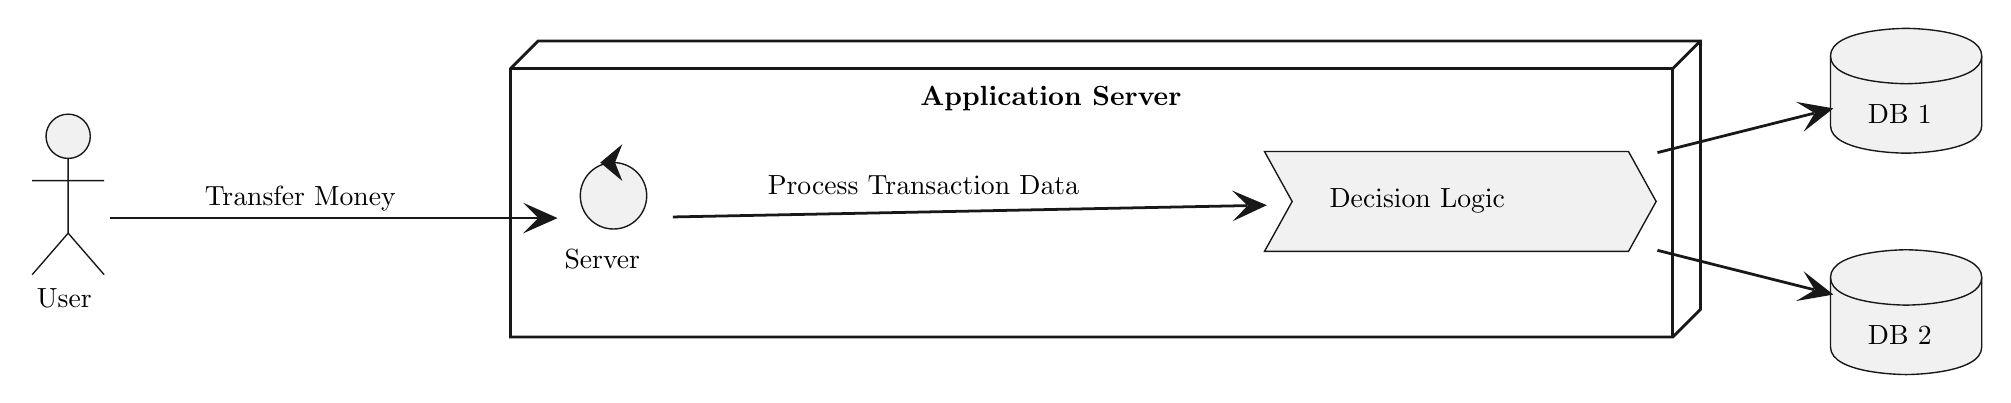
\begin{tikzpicture}[yscale=-1
        ,pstyle0/.style={color=plantucolor0000,line width=1.0pt}
        ,pstyle1/.style={color=plantucolor0000,fill=plantucolor0002,line width=0.5pt}
        ,pstyle2/.style={color=plantucolor0000,fill=plantucolor0000,line width=1.0pt}
        ,pstyle3/.style={color=plantucolor0000,line width=0.5pt}
        ]
        \draw[pstyle0] (180.66pt,20.55pt) -- (190.66pt,10.55pt) -- (610.64pt,10.55pt) -- (610.64pt,107.55pt) -- (600.64pt,117.55pt) -- (180.66pt,117.55pt) -- (180.66pt,20.55pt) -- cycle;
        \draw[pstyle0] (600.64pt,20.55pt) -- (610.64pt,10.55pt);
        \draw[pstyle0] (180.66pt,20.55pt) -- (600.64pt,20.55pt);
        \draw[pstyle0] (600.64pt,20.55pt) -- (600.64pt,117.55pt);
        \node at (325.2149pt,23.55pt)[below right,color=black]{\textbf{Application Server}};
        \draw[pstyle1] (217.887pt,66.5pt) ellipse (12pt and 12pt);
        \draw[pstyle2] (213.887pt,54.5pt) -- (219.887pt,49.5pt) -- (217.887pt,54.5pt) -- (219.887pt,59.5pt) -- (213.887pt,54.5pt) -- cycle;
        \node at (196.66pt,82.5pt)[below right,color=black]{Server};
        \draw[pstyle1] (453.12pt,50.5pt) -- (584.6456pt,50.5pt) -- (594.6456pt,68.5493pt) -- (584.6456pt,86.5986pt) -- (453.12pt,86.5986pt) -- (463.12pt,68.5493pt) -- cycle;
        \node at (473.12pt,60.5pt)[below right,color=black]{Decision Logic};
        \draw[pstyle1] (20.8308pt,45pt) ellipse (8pt and 8pt);
        \draw[pstyle3] (20.8308pt,53pt) -- (20.8308pt,80pt)(7.8308pt,61pt) -- (33.8308pt,61pt)(20.8308pt,80pt) -- (7.8308pt,95pt)(20.8308pt,80pt) -- (33.8308pt,95pt);
        \node at (6pt,96.5pt)[below right,color=black]{User};
        \draw[pstyle1] (657.64pt,16pt) ..controls (657.64pt,6pt) and (684.9733pt,6pt) .. (684.9733pt,6pt) ..controls (684.9733pt,6pt) and (712.3067pt,6pt) .. (712.3067pt,16pt) -- (712.3067pt,41.0986pt) ..controls (712.3067pt,51.0986pt) and (684.9733pt,51.0986pt) .. (684.9733pt,51.0986pt) ..controls (684.9733pt,51.0986pt) and (657.64pt,51.0986pt) .. (657.64pt,41.0986pt) -- (657.64pt,16pt);
        \draw[pstyle3] (657.64pt,16pt) ..controls (657.64pt,26pt) and (684.9733pt,26pt) .. (684.9733pt,26pt) ..controls (684.9733pt,26pt) and (712.3067pt,26pt) .. (712.3067pt,16pt);
        \node at (667.64pt,30pt)[below right,color=black]{DB 1};
        \draw[pstyle1] (657.64pt,96pt) ..controls (657.64pt,86pt) and (684.9733pt,86pt) .. (684.9733pt,86pt) ..controls (684.9733pt,86pt) and (712.3067pt,86pt) .. (712.3067pt,96pt) -- (712.3067pt,121.0986pt) ..controls (712.3067pt,131.0986pt) and (684.9733pt,131.0986pt) .. (684.9733pt,131.0986pt) ..controls (684.9733pt,131.0986pt) and (657.64pt,131.0986pt) .. (657.64pt,121.0986pt) -- (657.64pt,96pt);
        \draw[pstyle3] (657.64pt,96pt) ..controls (657.64pt,106pt) and (684.9733pt,106pt) .. (684.9733pt,106pt) ..controls (684.9733pt,106pt) and (712.3067pt,106pt) .. (712.3067pt,96pt);
        \node at (667.64pt,110pt)[below right,color=black]{DB 2};
        \draw[pstyle0] (35.86pt,74.55pt) ..controls (69.84pt,74.55pt) and (150.68pt,74.55pt) .. (190.45pt,74.55pt);
        \draw[pstyle2] (196.45pt,74.55pt) -- (187.45pt,70.55pt) -- (191.45pt,74.55pt) -- (187.45pt,78.55pt) -- (196.45pt,74.55pt) -- cycle;
        \node at (66.66pt,59.55pt)[below right,color=black]{Transfer Money};
        \draw[pstyle0] (239.31pt,74.15pt) ..controls (282.24pt,73.3pt) and (377.5912pt,71.4188pt) .. (446.7412pt,70.0488pt);
        \draw[pstyle2] (452.74pt,69.93pt) -- (443.6625pt,66.1091pt) -- (447.741pt,70.029pt) -- (443.821pt,74.1075pt) -- (452.74pt,69.93pt) -- cycle;
        \node at (270.12pt,55.66pt)[below right,color=black]{Process Transaction Data};
        \draw[pstyle0] (595.12pt,50.89pt) ..controls (617.27pt,45.32pt) and (634.5609pt,40.9724pt) .. (651.6709pt,36.6724pt);
        \draw[pstyle2] (657.49pt,35.21pt) -- (647.7865pt,33.5243pt) -- (652.6408pt,36.4287pt) -- (649.7364pt,41.283pt) -- (657.49pt,35.21pt) -- cycle;
        \draw[pstyle0] (595.12pt,86.21pt) ..controls (617.27pt,91.78pt) and (634.5609pt,96.1276pt) .. (651.6709pt,100.4276pt);
        \draw[pstyle2] (657.49pt,101.89pt) -- (649.7364pt,95.817pt) -- (652.6408pt,100.6713pt) -- (647.7865pt,103.5757pt) -- (657.49pt,101.89pt) -- cycle;
        \end{tikzpicture}
    }

    \scalebox{2}{$\Downarrow$}

    \end{center}
    \scalebox{0.7}{After Configuration:}

    \begin{center}     
    \definecolor{plantucolor0000}{RGB}{24,24,24}
    \definecolor{plantucolor0001}{RGB}{0,0,0}
    \definecolor{plantucolor0002}{RGB}{241,241,241}
    \scalebox{0.4}{
        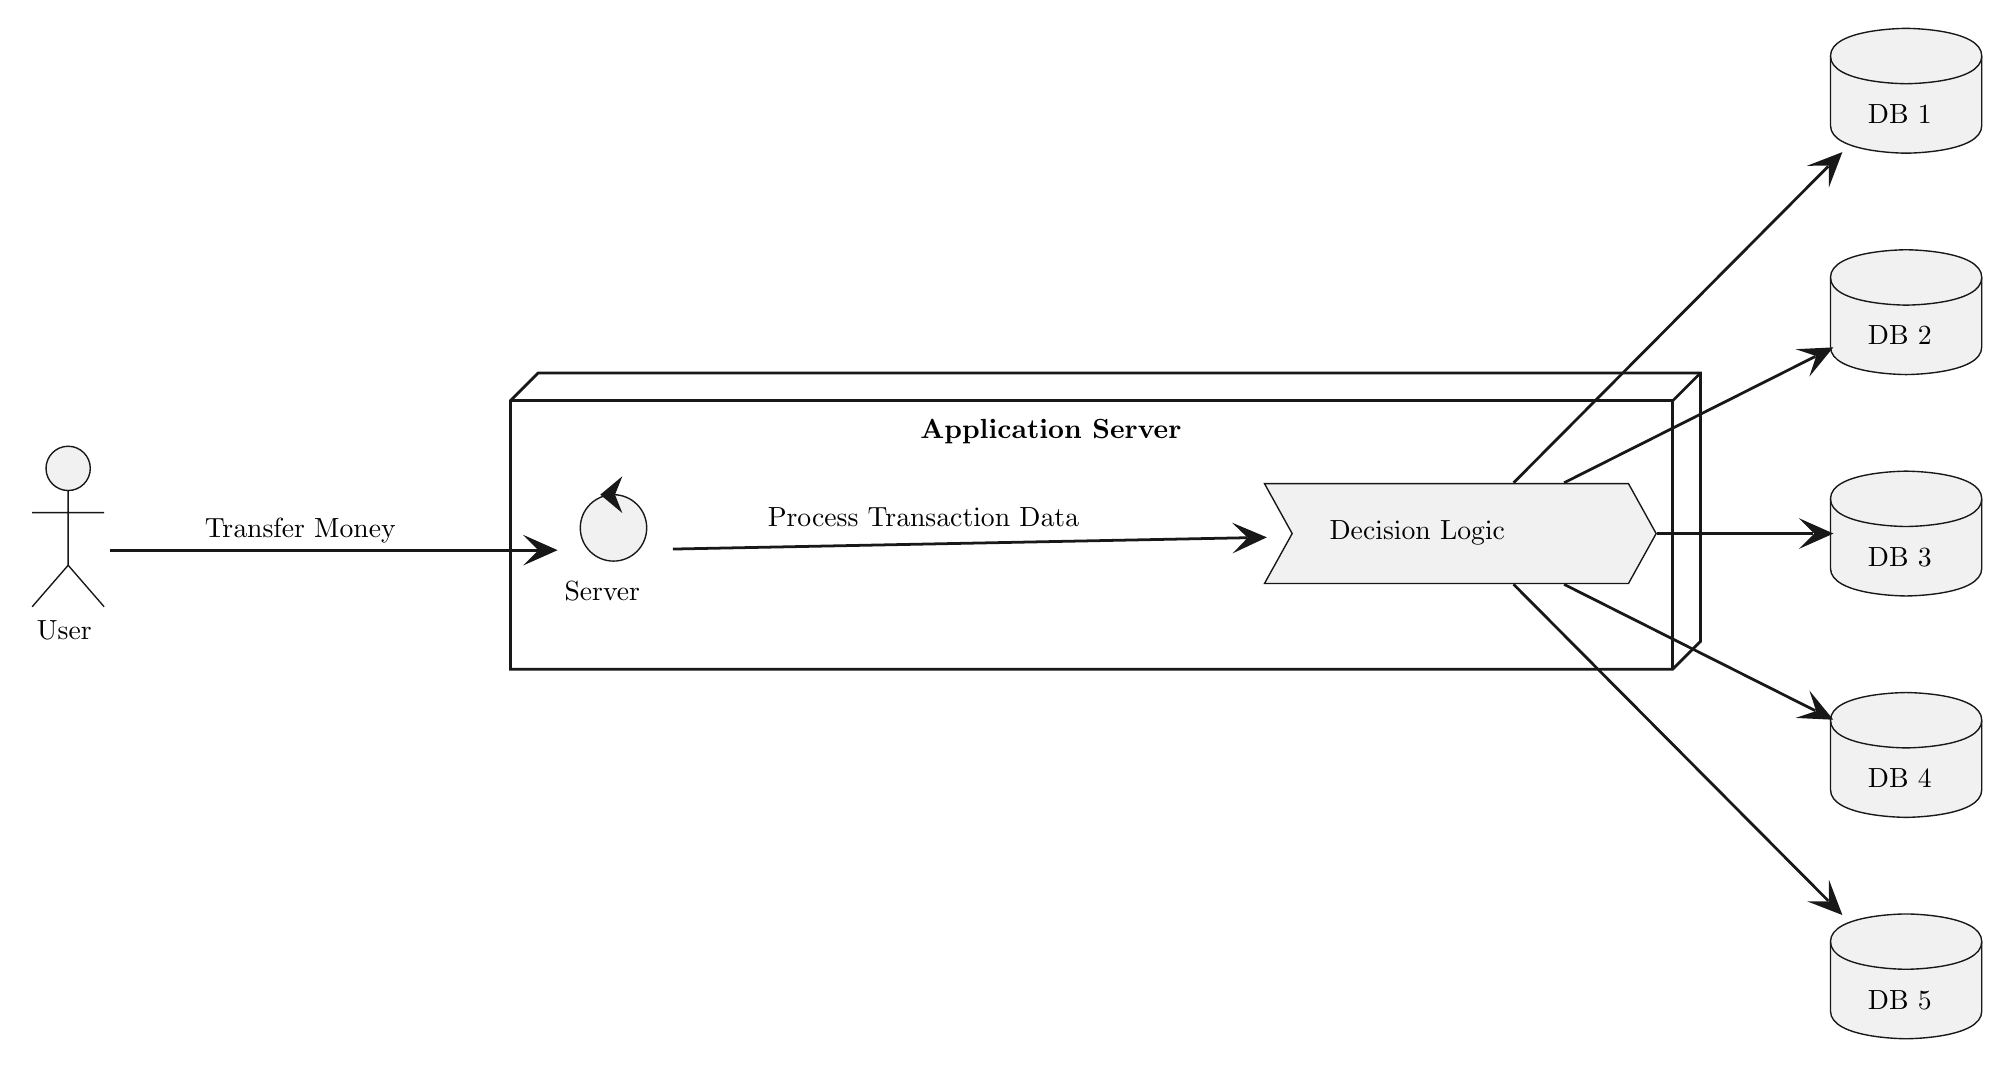
\begin{tikzpicture}[yscale=-1
        ,pstyle0/.style={color=plantucolor0000,line width=1.0pt}
        ,pstyle1/.style={color=plantucolor0000,fill=plantucolor0002,line width=0.5pt}
        ,pstyle2/.style={color=plantucolor0000,fill=plantucolor0000,line width=1.0pt}
        ,pstyle3/.style={color=plantucolor0000,line width=0.5pt}
        ]
        \draw[pstyle0] (180.66pt,140.55pt) -- (190.66pt,130.55pt) -- (610.64pt,130.55pt) -- (610.64pt,227.55pt) -- (600.64pt,237.55pt) -- (180.66pt,237.55pt) -- (180.66pt,140.55pt) -- cycle;
        \draw[pstyle0] (600.64pt,140.55pt) -- (610.64pt,130.55pt);
        \draw[pstyle0] (180.66pt,140.55pt) -- (600.64pt,140.55pt);
        \draw[pstyle0] (600.64pt,140.55pt) -- (600.64pt,237.55pt);
        \node at (325.2149pt,143.55pt)[below right,color=black]{\textbf{Application Server}};
        \draw[pstyle1] (217.887pt,186.5pt) ellipse (12pt and 12pt);
        \draw[pstyle2] (213.887pt,174.5pt) -- (219.887pt,169.5pt) -- (217.887pt,174.5pt) -- (219.887pt,179.5pt) -- (213.887pt,174.5pt) -- cycle;
        \node at (196.66pt,202.5pt)[below right,color=black]{Server};
        \draw[pstyle1] (453.12pt,170.5pt) -- (584.6456pt,170.5pt) -- (594.6456pt,188.5493pt) -- (584.6456pt,206.5986pt) -- (453.12pt,206.5986pt) -- (463.12pt,188.5493pt) -- cycle;
        \node at (473.12pt,180.5pt)[below right,color=black]{Decision Logic};
        \draw[pstyle1] (20.8308pt,165pt) ellipse (8pt and 8pt);
        \draw[pstyle3] (20.8308pt,173pt) -- (20.8308pt,200pt)(7.8308pt,181pt) -- (33.8308pt,181pt)(20.8308pt,200pt) -- (7.8308pt,215pt)(20.8308pt,200pt) -- (33.8308pt,215pt);
        \node at (6pt,216.5pt)[below right,color=black]{User};
        \draw[pstyle1] (657.64pt,16pt) ..controls (657.64pt,6pt) and (684.9733pt,6pt) .. (684.9733pt,6pt) ..controls (684.9733pt,6pt) and (712.3067pt,6pt) .. (712.3067pt,16pt) -- (712.3067pt,41.0986pt) ..controls (712.3067pt,51.0986pt) and (684.9733pt,51.0986pt) .. (684.9733pt,51.0986pt) ..controls (684.9733pt,51.0986pt) and (657.64pt,51.0986pt) .. (657.64pt,41.0986pt) -- (657.64pt,16pt);
        \draw[pstyle3] (657.64pt,16pt) ..controls (657.64pt,26pt) and (684.9733pt,26pt) .. (684.9733pt,26pt) ..controls (684.9733pt,26pt) and (712.3067pt,26pt) .. (712.3067pt,16pt);
        \node at (667.64pt,30pt)[below right,color=black]{DB 1};
        \draw[pstyle1] (657.64pt,96pt) ..controls (657.64pt,86pt) and (684.9733pt,86pt) .. (684.9733pt,86pt) ..controls (684.9733pt,86pt) and (712.3067pt,86pt) .. (712.3067pt,96pt) -- (712.3067pt,121.0986pt) ..controls (712.3067pt,131.0986pt) and (684.9733pt,131.0986pt) .. (684.9733pt,131.0986pt) ..controls (684.9733pt,131.0986pt) and (657.64pt,131.0986pt) .. (657.64pt,121.0986pt) -- (657.64pt,96pt);
        \draw[pstyle3] (657.64pt,96pt) ..controls (657.64pt,106pt) and (684.9733pt,106pt) .. (684.9733pt,106pt) ..controls (684.9733pt,106pt) and (712.3067pt,106pt) .. (712.3067pt,96pt);
        \node at (667.64pt,110pt)[below right,color=black]{DB 2};
        \draw[pstyle1] (657.64pt,176pt) ..controls (657.64pt,166pt) and (684.9733pt,166pt) .. (684.9733pt,166pt) ..controls (684.9733pt,166pt) and (712.3067pt,166pt) .. (712.3067pt,176pt) -- (712.3067pt,201.0986pt) ..controls (712.3067pt,211.0986pt) and (684.9733pt,211.0986pt) .. (684.9733pt,211.0986pt) ..controls (684.9733pt,211.0986pt) and (657.64pt,211.0986pt) .. (657.64pt,201.0986pt) -- (657.64pt,176pt);
        \draw[pstyle3] (657.64pt,176pt) ..controls (657.64pt,186pt) and (684.9733pt,186pt) .. (684.9733pt,186pt) ..controls (684.9733pt,186pt) and (712.3067pt,186pt) .. (712.3067pt,176pt);
        \node at (667.64pt,190pt)[below right,color=black]{DB 3};
        \draw[pstyle1] (657.64pt,256pt) ..controls (657.64pt,246pt) and (684.9733pt,246pt) .. (684.9733pt,246pt) ..controls (684.9733pt,246pt) and (712.3067pt,246pt) .. (712.3067pt,256pt) -- (712.3067pt,281.0986pt) ..controls (712.3067pt,291.0986pt) and (684.9733pt,291.0986pt) .. (684.9733pt,291.0986pt) ..controls (684.9733pt,291.0986pt) and (657.64pt,291.0986pt) .. (657.64pt,281.0986pt) -- (657.64pt,256pt);
        \draw[pstyle3] (657.64pt,256pt) ..controls (657.64pt,266pt) and (684.9733pt,266pt) .. (684.9733pt,266pt) ..controls (684.9733pt,266pt) and (712.3067pt,266pt) .. (712.3067pt,256pt);
        \node at (667.64pt,270pt)[below right,color=black]{DB 4};
        \draw[pstyle1] (657.64pt,336pt) ..controls (657.64pt,326pt) and (684.9733pt,326pt) .. (684.9733pt,326pt) ..controls (684.9733pt,326pt) and (712.3067pt,326pt) .. (712.3067pt,336pt) -- (712.3067pt,361.0986pt) ..controls (712.3067pt,371.0986pt) and (684.9733pt,371.0986pt) .. (684.9733pt,371.0986pt) ..controls (684.9733pt,371.0986pt) and (657.64pt,371.0986pt) .. (657.64pt,361.0986pt) -- (657.64pt,336pt);
        \draw[pstyle3] (657.64pt,336pt) ..controls (657.64pt,346pt) and (684.9733pt,346pt) .. (684.9733pt,346pt) ..controls (684.9733pt,346pt) and (712.3067pt,346pt) .. (712.3067pt,336pt);
        \node at (667.64pt,350pt)[below right,color=black]{DB 5};
        \draw[pstyle0] (35.86pt,194.55pt) ..controls (69.84pt,194.55pt) and (150.68pt,194.55pt) .. (190.45pt,194.55pt);
        \draw[pstyle2] (196.45pt,194.55pt) -- (187.45pt,190.55pt) -- (191.45pt,194.55pt) -- (187.45pt,198.55pt) -- (196.45pt,194.55pt) -- cycle;
        \node at (66.66pt,179.55pt)[below right,color=black]{Transfer Money};
        \draw[pstyle0] (239.31pt,194.15pt) ..controls (282.24pt,193.3pt) and (377.5912pt,191.418pt) .. (446.7412pt,190.058pt);
        \draw[pstyle2] (452.74pt,189.94pt) -- (443.6631pt,186.1177pt) -- (447.741pt,190.0383pt) -- (443.8204pt,194.1162pt) -- (452.74pt,189.94pt) -- cycle;
        \node at (270.12pt,175.66pt)[below right,color=black]{Process Transaction Data};
        \draw[pstyle0] (543.13pt,170.2pt) ..controls (572.27pt,140.89pt) and (625.0193pt,87.8446pt) .. (656.8493pt,55.8346pt);
        \draw[pstyle2] (661.08pt,51.58pt) -- (651.8976pt,55.1414pt) -- (657.5544pt,55.1255pt) -- (657.5704pt,60.7823pt) -- (661.08pt,51.58pt) -- cycle;
        \draw[pstyle0] (561.38pt,170.2pt) ..controls (590.73pt,155.44pt) and (625.9196pt,137.7455pt) .. (652.2096pt,124.5255pt);
        \draw[pstyle2] (657.57pt,121.83pt) -- (647.7323pt,122.2996pt) -- (653.103pt,124.0763pt) -- (651.3264pt,129.4469pt) -- (657.57pt,121.83pt) -- cycle;
        \draw[pstyle0] (595.12pt,188.55pt) ..controls (617.27pt,188.55pt) and (634.38pt,188.55pt) .. (651.49pt,188.55pt);
        \draw[pstyle2] (657.49pt,188.55pt) -- (648.49pt,184.55pt) -- (652.49pt,188.55pt) -- (648.49pt,192.55pt) -- (657.49pt,188.55pt) -- cycle;
        \draw[pstyle0] (561.38pt,206.9pt) ..controls (590.73pt,221.67pt) and (625.9187pt,239.3661pt) .. (652.2087pt,252.5761pt);
        \draw[pstyle2] (657.57pt,255.27pt) -- (651.324pt,247.655pt) -- (653.1023pt,253.0251pt) -- (647.7322pt,254.8033pt) -- (657.57pt,255.27pt) -- cycle;
        \draw[pstyle0] (543.13pt,206.9pt) ..controls (572.27pt,236.21pt) and (625.0193pt,289.2554pt) .. (656.8493pt,321.2654pt);
        \draw[pstyle2] (661.08pt,325.52pt) -- (657.5704pt,316.3177pt) -- (657.5544pt,321.9745pt) -- (651.8976pt,321.9586pt) -- (661.08pt,325.52pt) -- cycle;
        \end{tikzpicture}
    }

    \end{center}
    \caption[Shared Database Configuration]{การเปลี่ยน Configration การเข้าถึงฐานข้อมูล}
    \label{fig:fababean}
\end{figure}

\subsection{\ifenglish User Management and Access Control with Keycloak\else งานการบริหารข้อมูลผู้ใช้งานและสิทธิการใช้งานด้วย Keycloak\fi}
ในโปรเจค xPlatform เดิมทีจะมีการจัดเก็บข้อมูลผู้ใช้และ Credential ภายในฐานข้อมูลของระบบเพียงอย่างเดียว ซึ่งทำให้เกิดความไม่สะดวกสำหรับผู้ใช้งานที่อยากเข้าถึง แอปพลิเคชั่นอื่น ๆ ที่อยู่ภายใต้การดูแลของบริษัทลูกค้า Integrated ไว้กับ xPlatform อย่างเช่น Jenkins ArgoCD Nexus หรือ SonarQube\enskip การที่ผู้ใช้ต้องล็อกอินซ้ำหลายครั้งกับแอปพลิเคชันต่าง ๆ ส่งผลให้เกิดประสบการณ์การใช้งานที่ไม่ราบรื่นและมีความซับซ้อนมากขึ้น ดังนั้น เพื่อแก้ไขปัญหานี้ เราจึงได้นำ Keycloak มาใช้ในการทำหน้าที่เป็น Identity Provider ทำให้แต่ละแอปพลิเคชันสามารถ Authenticate และ Authorize ผู้ใช้ผ่านบริการของ Keycloak เพียงอย่างเดียว

Keycloak เป็นซอฟต์แวร์ที่ทำหน้าที่ในการจัดการ Authentication และ Authorization ซึ่งมีจุดเด่นที่สำคัญในการทำ Single Sign-On (SSO) โดยช่วยให้ผู้ใช้ล็อกอินเพียงครั้งเดียวและสามารถเข้าถึงแอปพลิเคชันต่าง ๆ ได้โดยไม่ต้องทำการล็อกอินซ้ำ ซึ่งช่วยลดความซับซ้อนในการใช้งานและเพิ่มความสะดวกให้กับผู้ใช้เป็นอย่างมาก นอกจากนี้ Keycloak ยังทำให้การรวม Identity Provider หลาย ๆ ตัวเข้าด้วยกันเป็นเรื่องง่ายขึ้น

ในการจัดการข้อมูลผู้ใช้งาน ระบบของ Keycloak จะทำการแบ่ง Entity ออกเป็น 5 ประเภทหลัก ๆ ดังนี้
\begin{enumerate}
    \item \textbf{User:} เป็นตัวแทนของผู้ใช้งานแต่ละคนในระบบ
    \item \textbf{User Group:} คือกลุ่มของผู้ใช้งาน ซึ่งช่วยให้ง่ายต่อการกำหนดสิทธิการใช้งานต่าง ๆ โดยสามารถกำหนดสิทธิให้กับกลุ่มผู้ใช้ได้แทนการตั้งค่าเป็นรายบุคคล
    \item \textbf{Client:} คือตัวแทนของ Services ต่าง ๆ เช่น Jenkins หรือแม้แต่ xPlatform เอง
    \item \textbf{Role:} เป็นชุดสิทธิการใช้งานที่ระบุถึงการเข้าถึงหรือการทำงานที่กลุ่มผู้ใช้สามารถทำได้ โดย Role จะแบ่งออกเป็นสองประเภท ได้แก่ Client Role ซึ่งเชื่อมโยงกับบริการเฉพาะ และ Realm Role
    \item \textbf{Realm:} คือ การแบ่งพื้นที่ในระบบออกเป็นส่วน ๆ เพื่อจัดการ User Group, Role และ Client ให้เกาะกันเป็นกลุ่ม
\end{enumerate}
นอกจากนี้ xPlatform มีการแบ่งหน้าที่ความรับผิดชอบออกเป็น 3 ระดับ ดังนี้:

\begin{enumerate}
    \item \textbf{ระดับ Company}: จะมีการสร้าง Realm และ Client สำหรับแต่ละบริษัท 
    \item \textbf{ระดับ Project}: จะมีการกำหนด Client Roles, Realm Roles และ User Groups สำหรับแต่ละโปรเจค เพื่อควบคุมการเข้าถึงและการกำหนดสิทธิของผู้ใช้งาน
    \item \textbf{ระดับ User}: มีหน้าที่สร้างผู้ใช้งานในแต่ละ Realm และเชื่อมโยงผู้ใช้เหล่านั้นเข้ากับ User Group ที่เกี่ยวข้องกับโปรเจค เมื่อมีการเพิ่มผู้ใช้งานในโปรเจค
\end{enumerate}
\begin{figure}[H]
    \begin{center}
        \includegraphics[scale=0.29]{resources/keycloak-er.png}
    \end{center}
    \caption[แบบจำลองความมสัมพันธ์ระหว่างข้อมูลภายใน Keycloak แบบย่อ]{แบบจำลองความมสัมพันธ์ระหว่างข้อมูลภายใน Keycloak แบบย่อ}
    \label{fig:keycloak-er}
\end{figure}
\textit{หมายเหตุ: ทุก ๆ Entity ในแบบจำลองความสัมพันธ์ ยกเว้น Realm นั้น มีความสัมพันธ์กับ Realm แบบ many-to-one แต่เส้นแสดงความสัมพันธ์ถูกตัดทอนออกเพื่อให้สามารถทำความเข้าใจได้ง่ายขึ้น}

แต่ละ Services สามารถทำการ Authenticate ด้วยการใช้ Token จากผู้ใช้งานที่ได้มาจากการล็อกอินด้วย Keycloak ซึ่งใน Token นี้จะประกอบข้อมูลที่ช่วยในการสืบค้น Role ได้ อย่างเช่น User Group หรือ Realm Role แล้วแต่ว่า Keycloak นั้นถูกตั้งค่ามาอย่างไร ซึ่งแต่ละ Service ก็จะสามารถยืนยัน Role ผ่านตัวของ Client ใน Keycloak ก่อนที่จะดูว่า Role ที่ผู้ใช้งานมีอยู่นั้น สามารถใช้สิทธิอะไรได้บ้างบนตัวของ Service
\begin{figure}[H]
    \begin{center}
        \includegraphics[scale=0.19]{resources/authorization-diagram.png}
    \end{center}
    \caption[แบบจำลองการ Authorization กับ Authentication ผ่าน Keycloak]{แบบจำลองการ Authorization กับ Authentication ผ่าน Keycloak}
    \label{fig:authorization-diagram}
\end{figure}
ชุดสิทธิการใช้งานถูกแบ่งออกเป็น 2 ประเภทหลัก ได้แก่ Realm Role และ Client Role โดยการเลือกใช้งานแต่ละประเภทขึ้นอยู่กับ Service ที่พร้อมจะ Integrate กับ Keycloak อย่างไร ตัวอย่างเช่น Jenkins และ ArgoCD จะอ้างอิงสิทธิการใช้งานจาก Realm Role ในขณะที่ Nexus และ SonarQube จะอ้างอิงจาก Client Role แทน

\subsection{\ifenglish xPlatform Custom Library Feature\else ฟีเจอร์ xPlatform Custom Library \fi}
ในระบบ xPlatform ผู้ใช้งานสามารถรวมโมดูลหลาย ๆ ส่วนเข้าด้วยกันเพื่อสร้างซอฟต์แวร์ขนาดใหญ่ขึ้น โดยโมดูลเหล่านี้มีบทบาทสำคัญในการเสริมสร้างความสามารถของระบบ ซอฟต์แวร์เหล่านี้สามารถแบ่งออกเป็น 4 ประเภทหลัก ได้แก่
\begin{enumerate} 
    \item \textbf{Service: } ส่วนที่ทำหน้าที่ประมวลผลหลัก ซึ่งมักจะเรียกว่าแอปพลิเคชัน  เป็นส่วนที่ผู้ใช้งานหรือระบบอื่น ๆ สามารถสื่อสารหรือทำงานร่วมกับซอฟต์แวร์ได้
    \item \textbf{Infrastructure: } หรือในบริบทนี้คือ Infrastructure as Code ซึ่งไว้สำหรับการจัดเตรียมและการจัดการส่วนประกอบต่าง ๆ บนโครงสร้างพื้นฐานของแอปพลิเคชั่น
    \item \textbf{Secret: } ส่วนที่เกี่ยวข้องกับการจัดเก็บข้อมูลที่มีความอ่อนไหว เช่น รหัสผ่านของผู้ใช้งาน โทเคน API หรือข้อมูลที่ต้องการความปลอดภัยสูง การจัดการกับข้อมูลเหล่านี้จะต้องมีการเข้ารหัสและการควบคุมการเข้าถึงอย่างเข้มงวดเพื่อป้องกันการรั่วไหลของข้อมูล 
    \item \textbf{Custom Library: } ส่วนของโค้ดที่ประกอบด้วยฟังก์ชันหรือ Definition ที่ถูกใช้งานบ่อย เพื่อให้ Services หลายตัวสามารถใช้งานร่วมกันได้โดยไม่ต้องเขียนโค้ดซ้ำ ๆ ในแต่ละ Service การใช้ Custom Library ช่วยลดความซับซ้อนและป้องกันการเกิด Code Duplication ซึ่งเป็นประโยชน์อย่างยิ่งสำหรับซอฟต์แวร์ที่ใช้สถาปัตยกรรมแบบ Microservice 
\end{enumerate}

ก่อนหน้านี้ xPlatform มีเพียง 3 ส่วนประกอบหลัก ได้แก่ Service Infrastructure และ Secret ซึ่งสามารถตอบโจทย์การใช้งานในระดับหนึ่ง ทีมพัฒนาได้มอบหมายงาน  ให้พัฒนาส่วนของ Custom Library เพิ่มเติม ส่วนประกอบนี้ถูกออกแบบมาเพื่อให้การใช้งานฟังก์ชันที่ใช้บ่อยมีความคล่องตัวมากขึ้น และช่วยให้กระบวนการพัฒนาซอฟต์แวร์รวดเร็วขึ้นและลดภาระงานในการจัดการโค้ดในแต่ละ Service

การพัฒนาส่วนของ Custom Library นั้นมีหลายขั้นตอนที่คล้ายคลึงกับ Service โดยเริ่มจากการสร้าง Repository ใหม่สำหรับจัดเก็บโค้ด และการสั่ง Build โค้ด ซึ่งเปรียบเสมือนการแปลงโค้ดให้อยู่ในรูปแบบที่คอมพิวเตอร์สามารถเข้าใจและประมวลผลได้ (คล้ายกับการ Compile ในภาษาโปรแกรม เช่น C++ หรือ Java) อย่างไรก็ตาม Custom Library แตกต่างจาก Service ตรงที่ว่าเมื่อพัฒนาเสร็จสิ้นแล้วจะไม่มีการ Deploy เนื่องจาก Custom Library ไม่จำเป็นต้องเปิดให้ระบบอื่น ๆ แต่จะถูกฝังภายในโค้ดของ Service ต่าง ๆ ที่เรียกใช้งานแทน

\subsection{\ifenglish xPlatform Documentation Feature\else ฟีเจอร์ xPlatform Documentation \fi}
ฟีเจอร์นี้เป็นฟีเจอร์ที่ถูกพัฒนาขึ้นมาเพื่อค้นหาและดึงข้อมูลจากไฟล์ Markdown ที่อยู่ใน Repositories ต่าง ๆ อย่าง  Service หรือ Custom Library บนแพลตฟอร์ม GitLab ฟีเจอร์นี้จะช่วยให้สามารถค้นหาไฟล์ Markdown เมื่อฟีเจอร์นี้ค้นพบไฟล์ Markdown ที่เกี่ยวข้องแล้ว ระบบจะทำการดึงเนื้อหาภายในไฟล์เหล่านั้นมาแสดงในหน้าเว็บเพจ ทั้งนี้เพื่อช่วยให้ผู้ใช้งานสามารถอ่าน Documentation ของแต่ละ Repository ผ่านเว็บไซต์ของ xPlatform ได้โดยไม่จำเป็นต้องเข้าไปอ่านใน GitLab

\section{\ifenglish Software Architecture and Infrastructures\else โครงสร้างพื้นฐานและสถาปัตยกรรมของซอฟต์แวร์ \fi}
\subsection{\ifenglish Software Architecture and Infrastructures of xPlatform\else โครงสร้างพื้นฐานและสถาปัตยกรรมของซอฟต์แวร์โปรเจค xPlatform\fi}
xPlatform เป็นโปรเจค Full-Stack ที่ใช้สถาปัตยกรรมแบบ Microservice
\begin{enumerate}
    \item หลังบ้าน
    \begin{enumerate}
        \item \textbf{ExpressJS (Typescript):} เป็นเฟรมเวิร์คสำหรับการพัฒนาเว็บแอปพลิเคชันฝั่งเซิร์ฟเวอร์ที่ใช้ Node.js โดย ExpressJS มีความยืดหยุ่นสูงและสามารถสร้าง API ได้อย่างรวดเร็ว ส่วนการใช้ Typescript ช่วยเพิ่มความปลอดภัยในการเขียนโค้ดด้วยการตรวจสอบประเภทของข้อมูล (Type Checking) ทำให้โค้ดมีความเสถียรและลดข้อผิดพลาด
        \item \textbf{Apollo GraphQL:} เป็นไลบรารีสำหรับการใช้งาน GraphQL ซึ่งเป็นภาษาสำหรับการดึงข้อมูลจากเซิร์ฟเวอร์ โดย Apollo GraphQL สามารถช่วยให้ฝั่งเรียกใช้ API มีความสะดวกมากขึ้น โดยเฉพาะเมื่อใช้ในสถาปัตยกรรมไมโครเซอร์วิส ซึ่งช่วยให้สามารถจัดการการดึงข้อมูลจากบริการหลาย ๆ แหล่ง
        \begin{enumerate}
            \item การควบคุมประเภทข้อมูล (Controlled Type) GraphQL ช่วยให้สามารถกำหนดประเภทของข้อมูลที่ส่งและรับได้อย่างชัดเจน ซึ่งช่วยลดข้อผิดพลาดในการส่งข้อมูลที่ไม่ตรงตามประเภทที่กำหนด และเพิ่มความปลอดภัยในการใช้งาน TODO: refernce apollo Type
            
            \textbf{ยกตัวอย่าง}
            \begin{center}                
                \begin{lstlisting}
getPosts(getPostsQuery: GetPostsQuery!): GetPostsResult!

input GetPostsQuery {
  ownerId: String!
  searchQuery: String
  afterDate: Date
}

type GetPostsResult {
  posts: [Post]!
  owner: User
}

type User {
  userId: String!
  username: String!
  posts: [Post]!
  comments: [Comment]!
}

type Post {
  postId: String!
  content: String!
  owner: User
  replies: [Comment]!
}
                \end{lstlisting}
            \end{center}
            ในตัวอย่างนี้ API ที่ชื่อว่า {\tt getPosts} จะรับข้อมูลเข้าในรูปของ {\tt GetPostsQuery} และจะส่งข้อมูลกลับในรูปของ {\tt GetPostsResult} โดยที่เครื่องหมาย \texttt{[]} หมายถึงข้อมูลประเภทอาเรย์ และ เครื่องหมาย \texttt{!} หมายถึงฟิลด์นั้น ๆ เป็น non-nullable ซึ่งหมายความว่าฟิลด์ต้องมีค่าภายในทุกครั้งที่มีการส่งข้อมูล ไม่สามารถเป็น \texttt{null} ได้

            \item ฝั่งเรียกใช้ API สามารถเลือกข้อมูลที่จำเป็นต่อการใช้งานได้ยืดหยุ่น นอกจากนี้ยังสามารถเลือกข้อมูลภายในที่เป็น Object ได้ เช่น ผู้ใช้ที่เรียกใช้งาน \texttt{getPosts} จะสามารถเลือกข้อมูลใด ๆ ใน \texttt{GetPostsQuery} ได้ตามต้องการ นอกจากนี้ยังสามารถค้นหาข้อมูลอื่น ๆ ภายใน \texttt{posts} และ \texttt{owner} ได้อีกด้วย TODO: refernce apollo Resolver
            
            \textbf{ยกตัวอย่าง}
            \begin{center}                
                \begin{lstlisting}
getPosts {
    posts {
        owner {
            username
        }
    }
    owner {
        posts {
            content
        }
    }
}
                \end{lstlisting}
            \end{center}
            ในตัวอย่างนี้ ผู้ใช้งานขอค้นหาข้อมูล \texttt{posts} และ \texttt{owner} จากข้อมูลประเภท \texttt{GetPostsResult}
            \begin{enumerate}
                \item ฟิลด์ \texttt{posts} จะดึงข้อมูลเกี่ยวกับผู้โพสต์ (owner) และในส่วนของ \texttt{owner} จะทำการค้นหาชื่อผู้ใช้ (username)
                \item ฟิลด์ \texttt{owner} จะเรียกดูโพสต์ (post) ทั้งหมดที่ผู้ใช้นั้นสร้างขึ้น และภายในแต่ละโพสต์จะค้นหาเนื้อหาที่เกี่ยวข้อง
            \end{enumerate}
           
           \item การรวม API ด้วย Apollo Federation คือการสร้าง service ที่สามารถ reroute requests ไปยัง service อื่น ๆ ซึ่งหมายความว่าผู้ใช้สามารถส่ง API request ไปยัง service ใด ๆ ก็ได้ผ่าน router TODO: reference Apollo Federation

           \item Apollo Federation ยังมีฟีเจอร์ Reference Resolver ซึ่งช่วยในการค้นหาข้อมูลของ Objects ที่อยู่ใน service ที่แตกต่างกัน ตัวอย่างเช่น ``post" service มีการเก็บข้อมูลของทุก ๆ โพสต์และคอมเมนต์ แต่ข้อมูลของผู้ใช้แต่ละคนจะถูกจัดการโดย ``user" service แทน\enskip Apollo Federation จะช่วยให้ใน API \texttt{getPost} ที่ถูกจัดการโดย ``post" service สามารถไปส่ง \texttt{userId} ให้ router ไปจัดการการดึงข้อมูล user จาก ``user" service ต่อโดยอัตโนมัติ TODO: reference resolveReference

        \end{enumerate}
    \end{enumerate}
    \item ตัวอย่างโครงสร้างพื้นฐานที่ใช้พัฒนา
    \begin{enumerate}
        \item \textbf{MySQL:} เป็นระบบจัดการฐานข้อมูลเชิงสัมพันธ์ ที่ใช้ภาษา SQL ในการสืบค้นและจัดการข้อมูล ซึ่ง MySQL เป็นระบบที่เหมาะสำหรับการจัดเก็บข้อมูลที่มีโครงสร้างชัดเจน และสามารถรองรับการทำงานร่วมกับแอปพลิเคชันต่าง ๆ
        \item \textbf{Jenkins:} เป็นเครื่องมือสำหรับการทำ Continuous Integration (CI) และ Continuous Delivery (CD) ซึ่งช่วยให้การพัฒนาและการปรับปรุงซอฟต์แวร์เป็นไปอย่างต่อเนื่องและอัตโนมัติ Jenkins สามารถทำการทดสอบและดีพลอยโค้ดได้อย่างรวดเร็ว ลดเวลาและข้อผิดพลาดในการพัฒนา
        \item \textbf{Keycloak: } เป็นซอฟต์แวร์ที่ทําหน้าที่ในการ Authentication ซึ่งมีจุดเด่นในการทํา Single Sign-On
        (SSO) ที่ช่วยให้ผู้ใช้สามารถล็อกอินเพียงครั้งเดียวและเข้าถึงแอปพลิเคชันอื่น ๆ ได้โดยไม่ต้องทําการล็อกอิน
        ซํ้า 
    \end{enumerate}
\end{enumerate}